\chapter{\IfLanguageName{dutch}{Stand van zaken}{State of the art}}%
\label{ch:stand-van-zaken}

% Tip: Begin elk hoofdstuk met een paragraaf inleiding die beschrijft hoe
% dit hoofdstuk past binnen het geheel van de bachelorproef. Geef in het
% bijzonder aan wat de link is met het vorige en volgende hoofdstuk.

% Pas na deze inleidende paragraaf komt de eerste sectiehoofding.
In dit hoofdstuk zullen we de basisprincipes van Swift en SwiftUI verkennen, samen met enkele essentiële design patterns en annotaties die vaak worden gebruikt in SwiftUI-ontwikkeling. De annotaties waar we het over gaan hebben zijn de annotaties die we gaan gebruiken om Data door te geven in SwiftUI. Na dit hoofdstuk heeft u genoeg kennis en inzicht om de rest van deze proef te begrijpen.


\section{Swift}
Swift is een programmeertaal ontwikkeld door Apple, primair bedoeld voor besturingssystemen zoals iOS, OS X, iPadOS, tvOS, en andere platforms van Apple. De taal vervangde de eerdere standaardtaal Objective-C voor app-ontwikkeling. Swift werd geïntroduceerd tijdens de jaarlijkse ontwikkelaarsconferentie WWDC 2014, samen met OS X Yosemite, iOS 8 en verschillende SDK's. Dit is de basis programmeertaal die we in deze proef zullen gebruiken.
\begin{figure}[H]
    \centering
    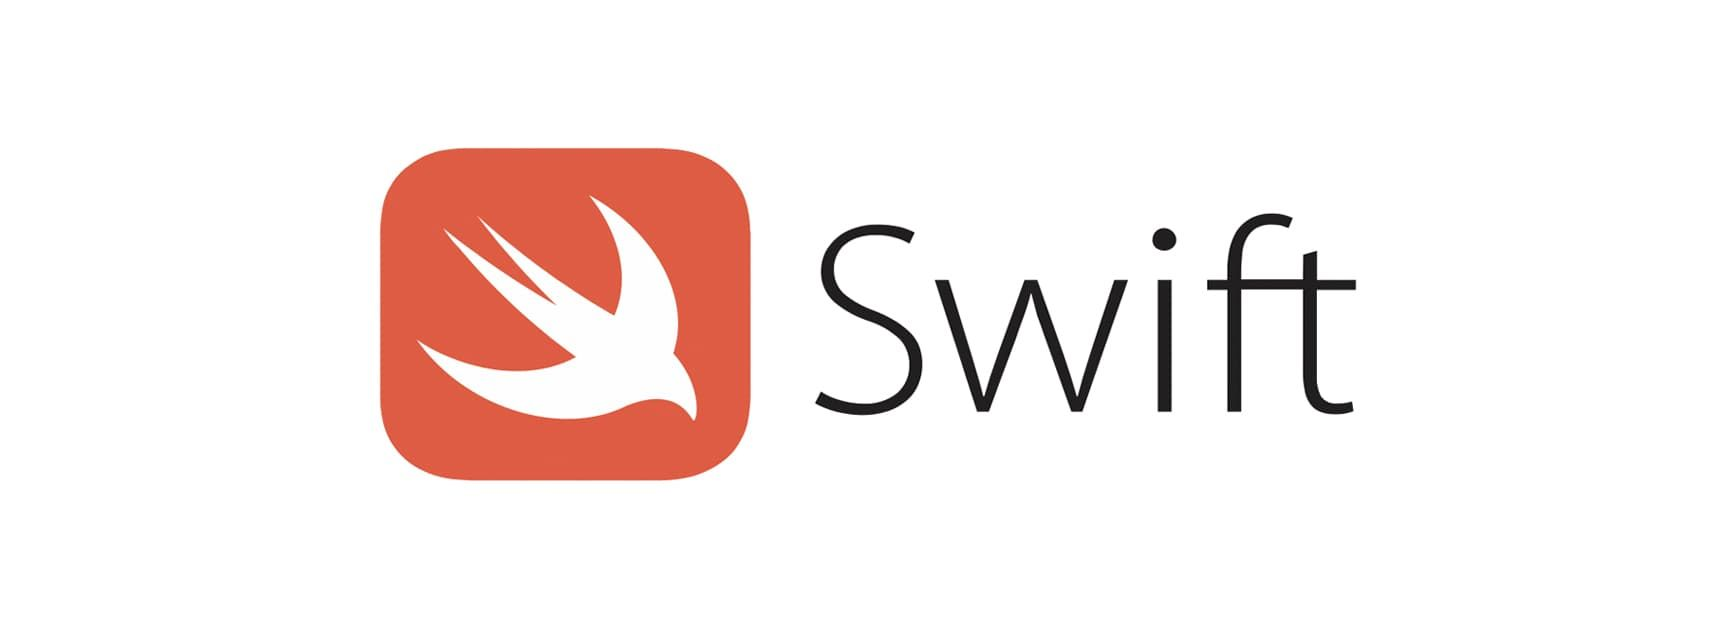
\includegraphics[width=0.4\textwidth]{swiftbird}
    \caption{Het Swift-logo \autocite{SwiftBirdImage}}
    \label{fig:swift}
\end{figure}

\subsubsection{Geschiedenis}
De ontwikkeling van Swift begon in 2010 onder leiding van programmeur Chris Lattner. De taal integreerde diverse concepten van andere programmeertalen, waaronder Objective-C, Rust, Haskell, Python, C-sharp, CLU, en meer. De eerste openbare Swift-app werd geschreven op 2 juni 2014.

Tijdens WWDC werd ook een handleiding van 500 pagina's beschikbaar gesteld via de iBooks Store en de website van Apple.
\section{SwiftUI}
\autocite{AppleSwiftUI} SwiftUI is een door Apple ontwikkeld framework voor het bouwen van gebruikersinterfaces voor iOS, macOS, watchOS en tvOS, met behulp van de programmeertaal Swift. Het is ontworpen om de ontwikkeling van gebruikersinterfaces te vereenvoudigen door middel van een declaratieve syntax en een reeks krachtige tools en functies. 
\begin{wrapfigure}{r}{0.3\textwidth}
    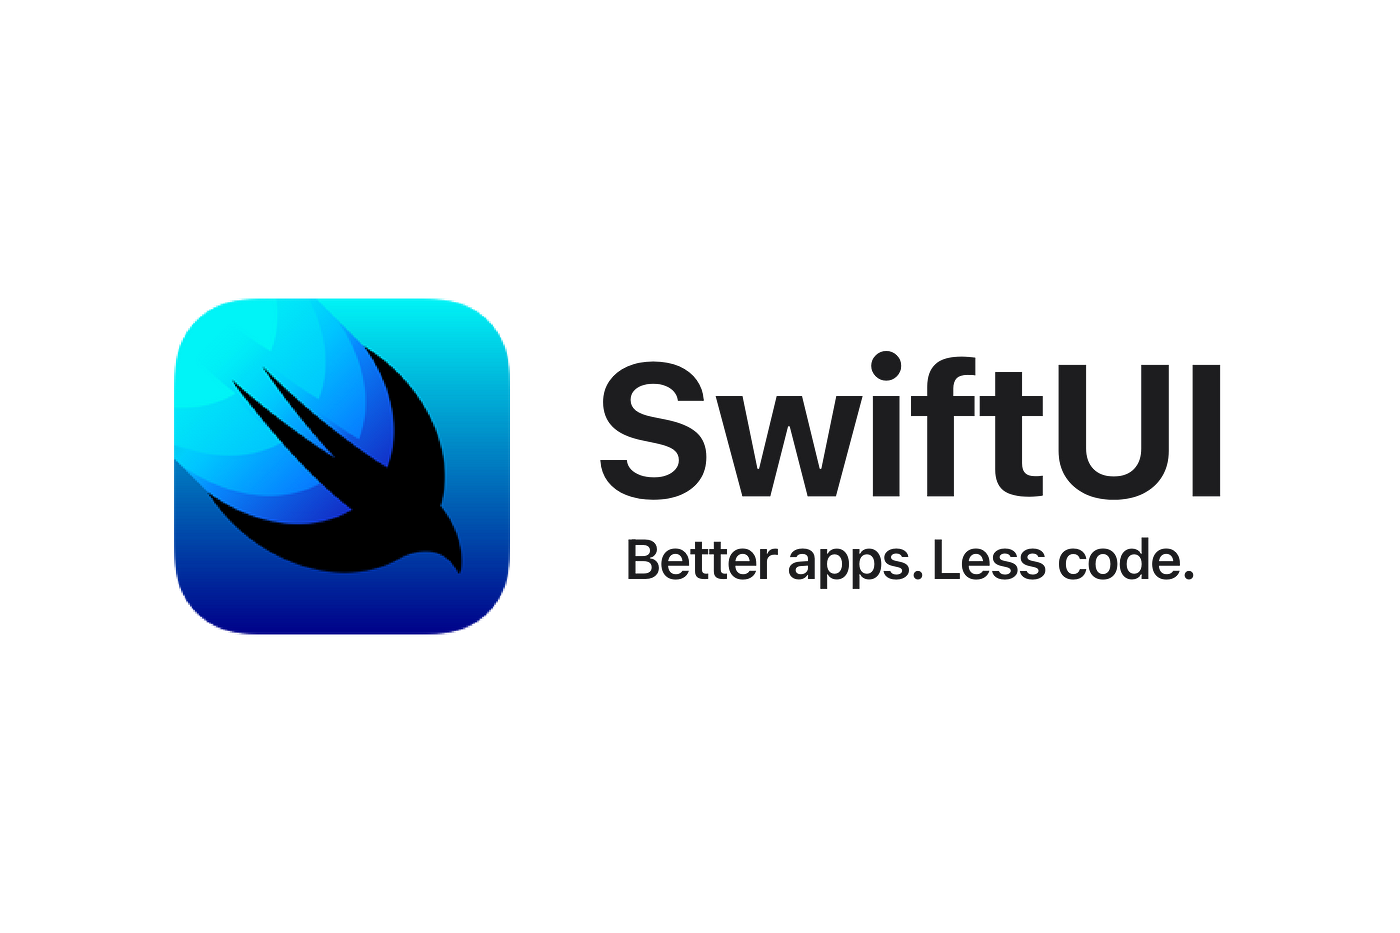
\includegraphics[width=0.3\textwidth]{swiftuibird} 
    \caption{Het swiftUI logo \autocite{SwiftUiImage}}
    \label{fig:swiftUI}
\end{wrapfigure}
Met SwiftUI kun je gebruikersinterfaces bouwen door middel van een reeks van herbruikbare en aanpasbare Views, waardoor je complexe UI-structuren kunt maken met minimale code. Het framework maakt gebruik van een state-driven architectuur, wat betekent dat de UI automatisch wordt bijgewerkt wanneer de toestand van de app verandert. SwiftUI vervangt UIKit als het primaire framework voor het bouwen van interfaces op Apple-platforms, maar het maakt achter de schermen nog steeds vaak gebruik van UIKit-componenten. In deze proef gaan we SwiftUI Views gebruiken om data aan mee te geven om zo performantie te tracken.


\subsection{Views}
\autocite{AppleSwiftViews} Views vormen de bouwstenen van elke SwiftUI-gebruikersinterface. Ze definiëren hoe content wordt weergegeven en gereageerd wordt op gebruikersinteracties. Views kunnen zowel elementaire interface-elementen (zoals tekst, knoppen en afbeeldingen) als complexere composities van deze elementen bevatten.

\begin{figure}[h]
    \begin{minipage}{0.5\textwidth}
        \begin{swift}[caption=Example of a view, label=view_example]
           struct MyView: View {
               var body: some View {
                   Text("Hello, World!")
               }
           }
        \end{swift}
    \end{minipage}%
    \hfill
    \begin{minipage}{0.45\textwidth}
        \centering
        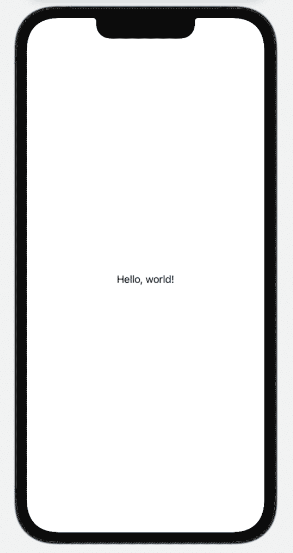
\includegraphics[height=130pt]{helloworldview}
        \caption{Example of a view}
        \label{fig:viewex1}
    \end{minipage}
\end{figure}

\subsection{VStack en HStack}
\autocite{AppleVstackHstack} VStack en HStack zijn eenvoudige en essentiële componenten in SwiftUI die helpen bij het organiseren van views in een user interface.

\textbf{VStack}: De VStack (Vertical Stack) positioneert views in een verticale lijn. Dit betekent dat elke view binnen een VStack onder de vorige wordt geplaatst, van boven naar beneden. Het is ideaal voor het maken van layouts waarbij je elementen verticaal wilt stapelen, zoals tekstblokken, afbeeldingen, knoppen, enzovoort.

\textbf{HStack}: De HStack (Horizontal Stack) positioneert views in een horizontale lijn. Dit betekent dat elke view binnen een HStack naast de vorige wordt geplaatst, van links naar rechts. HStack is nuttig voor het maken layouts waarbij je elementen naast elkaar wilt zetten, zoals een reeks knoppen naast elkaar, pictogrammen, of tekst met een afbeelding aan de zijkant.

\subsection{LazyVstack en LazyHstack}
\autocite{LazyHStackVStack} LazyVStack en LazyHStack zijn componenten in SwiftUI die vergelijkbaar zijn met VStack en HStack, maar ontworpen zijn voor efficiënter geheugen- en prestatiebeheer bij het weergeven van grote hoeveelheden data. 

\textbf{LazyVStack}: De LazyVStack (Lazy Vertical Stack) positioneert views in een verticale lijn, net als VStack. Het verschil is dat LazyVStack alleen de views rendert die momenteel zichtbaar zijn op het scherm. Dit betekent dat als je een lange lijst van items hebt, alleen de items binnen het zichtbare gedeelte van de lijst worden gerenderd en weergegeven, wat leidt tot betere prestaties en minder geheugengebruik.

\textbf{LazyHStack}: De LazyHStack (Lazy Horizontal Stack) positioneert views in een horizontale lijn, zoals HStack. Net als LazyVStack, rendert LazyHStack alleen de views die zichtbaar zijn in het scrollbare gebied. Dit maakt het mogelijk om efficiënte horizontale scrollable content te maken, zoals carrousels of galerijen met een groot aantal items.

\section{Design Patterns}
Design patterns zijn oplossingen voor veelvoorkomende ontwerpproblemen in softwareontwikkeling. Ze bieden gestandaardiseerde en herbruikbare oplossingen voor problemen die zich vaak voordoen tijdens het ontwerpen van software. In Swift met SwiftUI zijn verschillende design patterns van toepassing om de ontwikkeling van robuuste en onderhoudbare apps te vergemakkelijken.

Design Patterns zijn belangerijk voor:
\begin{itemize}
    \item {\textbf{Herbruikbaarheid:} Design patterns bevorderen herbruikbaarheid van code.}
    \item {\textbf{Onderhoudbaarheid:} Ze maken de code gemakkelijker te begrijpen en te onderhouden.}
    \item {\textbf{Schaalbaarheid:} Door het gebruik van design patterns wordt het gemakkelijker om de app uit te breiden en nieuwe functies toe te voegen.}
    \item {\textbf{Testbaarheid:} Code die gebruikmaakt van design patterns is vaak gemakkelijker te testen vanwege de modulaire structuur.}
\end{itemize}
\autocite{MediumPatterns} Enkele belangerijke Design Patterns in Swift met SwiftUI zijn MVVM, MVC, MVP en VIPER.

\subsection{Model-View-ViewModel (MVVM)}
\autocite{MediumMVVM} MVVM is een design pattern dat veel wordt gebruikt in SwiftUI voor het scheiden van de logica van de gebruikersinterface van de onderliggende gegevens. Het bestaat uit drie hoofdcomponenten:
\begin{figure}[H]
    \centering
    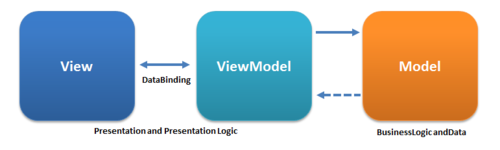
\includegraphics[width=1\textwidth]{MVVMPattern} 
    \caption{MVVM \autocite{MVVMImage}}
    \label{fig:mvvm}
\end{figure}
\begin{itemize}
    \item {\textbf{Model:} Het model bevat de gegevens van de app en de logica voor het manipuleren van die gegevens. Dit is waar de kernfunctionaliteit van de app zich bevindt.}
    \item {\textbf{View:} De view is verantwoordelijk voor het weergeven van de gebruikersinterface en het reageren op gebruikersinteracties. In SwiftUI worden views vaak passief gehouden en bevatten ze minimale logica.}
    \item {\textbf{ViewModel:} De viewmodel fungeert als een tussenliggende laag tussen het model en de view. Het voorziet de view van de gegevens die nodig zijn om te worden weergegeven en reageert op acties van de gebruiker. Het transformeert ook de gegevens van het model naar een vorm die gemakkelijk kan worden weergegeven in de view.}
\end{itemize}
De voordelen van MVVM zijn:
\begin{itemize}
    \item {\textbf{Scheiding van verantwoordelijkheden:} MVVM helpt bij het scheiden van de logica van de gebruikersinterface van de onderliggende gegevens, waardoor de code gemakkelijker te begrijpen en te onderhouden is. Dit zorgt ook voor een eenvoudigere uitbreidbaarheid en herbruikbaarheid van de code.}
    \item {\textbf{Testbaarheid:} Omdat de logica van de gebruikersinterface wordt gescheiden van de gegevenslogica, zijn de componenten gemakkelijker afzonderlijk te testen.}
        \item \textbf{Binding tussen View en ViewModel:} MVVM maakt gebruik van databinding om gegevens tussen de View en de ViewModel te synchroniseren, waardoor de code voor het bijwerken van de gebruikersinterface eenvoudiger en overzichtelijker wordt.
    
    \item \textbf{Flexibiliteit en schaalbaarheid:} Door de scheiding van verantwoordelijkheden kunnen verschillende teams parallel werken aan de ontwikkeling van de gebruikersinterface en de onderliggende gegevenslogica, wat de algehele flexibiliteit en schaalbaarheid van het project ten goede komt.
\end{itemize}

\subsection{VIPER}
\autocite{MediumVIPER} VIPER is een design pattern dat staat voor View, Interactor, Presenter, Entity, en Router. Het is een architectureel patroon dat is ontworpen om de code van een app in verschillende lagen te verdelen om de onderhoudbaarheid en testbaarheid te verbeteren. Hier is een overzicht van de componenten:
\begin{figure}[H]
    \centering
    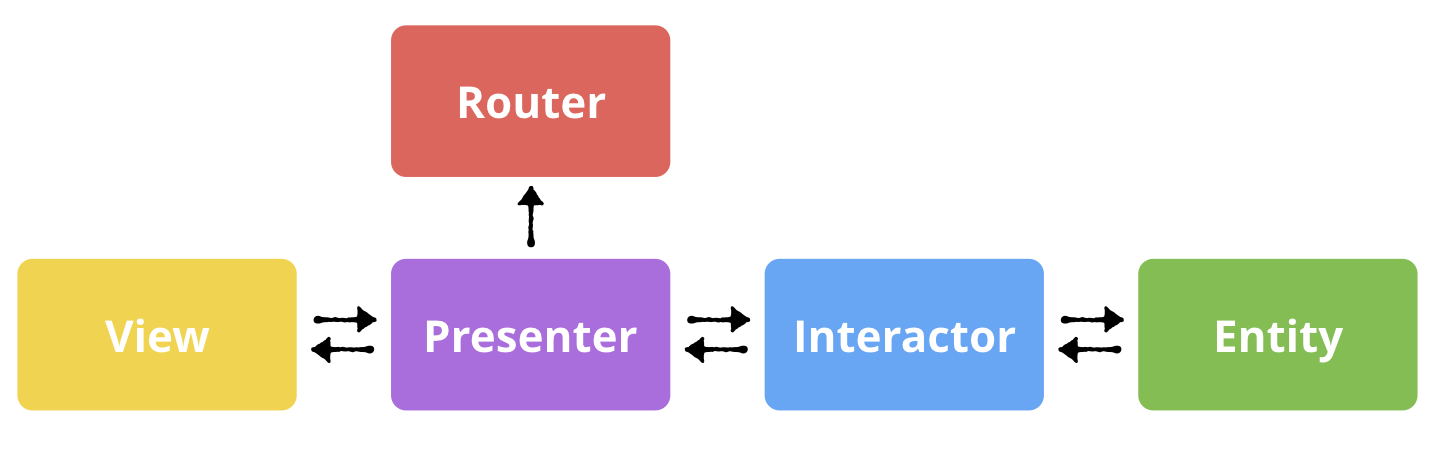
\includegraphics[width=1\textwidth]{viper} 
    \caption{viper \autocite{ViperImage}}
    \label{fig:viper}
\end{figure}

\begin{itemize}
    \item {\textbf{View:} De view is verantwoordelijk voor het weergeven van de gebruikersinterface en het reageren op gebruikersinteracties, vergelijkbaar met MVVM.}
    \item {\textbf{Interactor:} De interactorcomponent bevat de businesslogica van de app. Het is verantwoordelijk voor het ophalen en verwerken van gegevens van externe bronnen, zoals een database of een netwerk.}
    \item {\textbf{Presenter:} De presenter fungeert als een tussenliggende laag tussen de interactor en de view. Het is verantwoordelijk voor het formatteren van de gegevens die zijn verkregen van de interactor en deze door te geven aan de view voor weergave.}
    \item {\textbf{Entity:} De entity bevat de gegevensmodellen van de app. Het vertegenwoordigt de entiteiten die worden gebruikt in de applicatie, zoals gebruikers, items, of andere objecten.}
    \item {\textbf{Router:} De router is verantwoordelijk voor het beheren van de navigatie binnen de app. Het bepaalt welke schermen moeten worden weergegeven en hoe deze moeten worden genavigeerd.}
\end{itemize}
Voordelen van VIPER zijn:
\begin{itemize}
    \item {\textbf{Schaalbaarheid:} Door de code in verschillende lagen te verdelen, maakt VIPER het gemakkelijker om de app uit te breiden en nieuwe functies toe te voegen.}
    \item {\textbf{Testbaarheid:} Elk onderdeel van VIPER kan afzonderlijk worden getest, waardoor het gemakkelijker wordt om bugs op te sporen en te repareren.}
\end{itemize}

\section{XCode Performance Trackers}

In deze proef gericht op het vergelijken van de performantie, rendering en lifescycles van views, zijn Xcode Profiler, Xcode Instruments en XCTest Metrics van onschatbare waarde. Xcode Profiler biedt een basisprofiel van views door CPU-, geheugen- en netwerkactiviteit te meten. Xcode Instruments gaat dieper met gedetailleerde analyses van CPU-, geheugen- en grafische prestaties, en kan rendercycli traceren. XCMetrics biedt automatische verzameling van prestatiegegevens tijdens het uitvoeren van tests. Dit betekent dat tijdens het testen van de code, XCTest Metrics automatisch gegevens verzamelt over de prestaties van de app, waaronder informatie over de tijd die het kost om bepaalde taken uit te voeren, zoals het laden van views. Deze verzamelde gegevens kunnen worden geanalyseerd om prestatieproblemen in de views van de app te identificeren. Het integreren van bevindingen uit deze tools biedt een holistisch beeld van de view-prestaties, waardoor iteratieve optimalisatie mogelijk is voor een verbeterde gebruikerservaring en algehele app-prestaties.



\subsection{Xcode Instruments}
Xcode Instruments is een krachtige tool die wordt geleverd als onderdeel van Apple's Xcode-ontwikkelomgeving. Het stelt ontwikkelaars in staat om diepgaande analyses uit te voeren van de prestaties en het gedrag van hun iOS-, macOS-, watchOS- en tvOS-apps. Met Instruments kunnen ontwikkelaars problemen met prestaties, geheugen, energieverbruik en meer opsporen en diagnosticeren. 

\subsection{XCode Profiler}
Deze tool stelt ontwikkelaars in staat om de prestaties van hun iOS-, macOS-, watchOS- en tvOS-apps te meten en te optimaliseren. De profiler biedt inzicht in het runtime-gedrag van de app, inclusief CPU-gebruik, geheugenverbruik, netwerkactiviteit en meer. Met deze tool kunnen we in deze proef de performantie op basis van CPU-gebruik, geheugenverbruik, enz. gaan meten. 
\paragraph{CPU-profiler}
Hiermee kan men het CPU-gebruik van een app analyseren. Men kan zien welke delen van de code veel CPU-tijd verbruiken en mogelijk optimalisaties doorvoeren om de prestaties te verbeteren.
\begin{figure}[H]
    \centering
    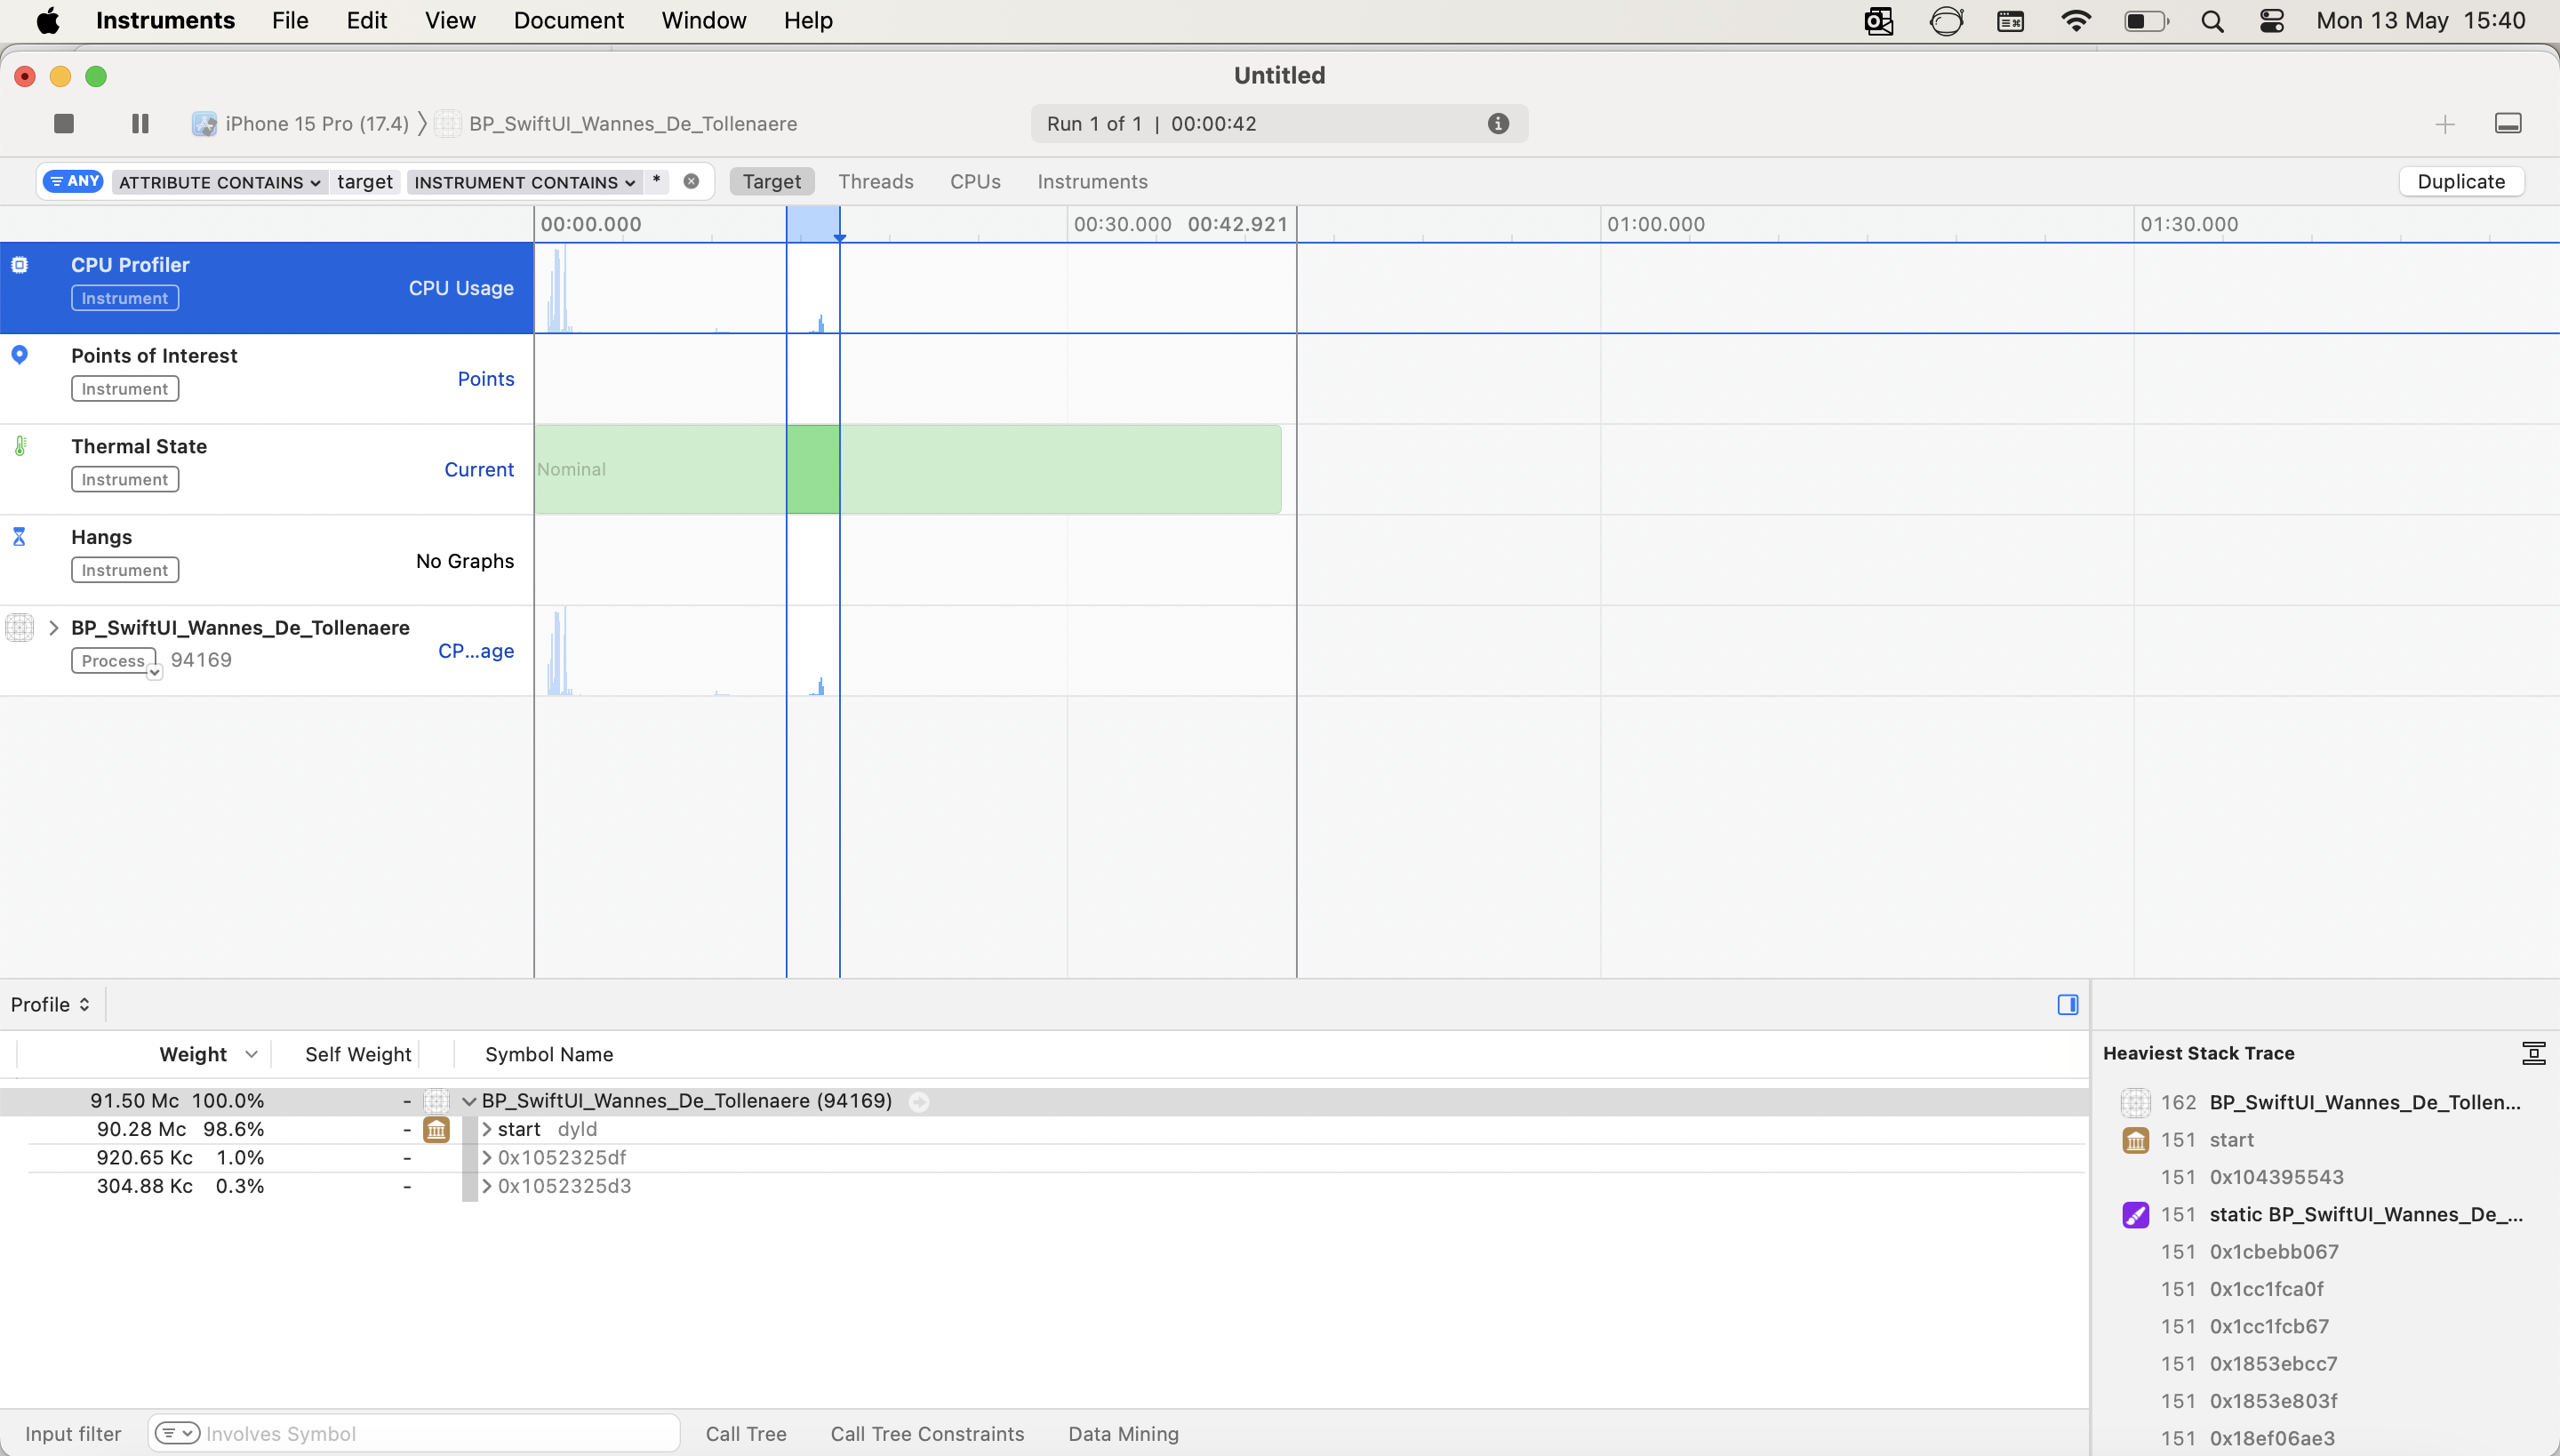
\includegraphics[width=1\textwidth]{BP_XcodeCpuProfiler} 
    \caption{Xcode CPU Profiler}
    \label{fig:cpuProfiler}
\end{figure}
\paragraph{Geheugen-profiler}
Hiermee kan men het geheugenverbruik van een app analyseren. Men kan zien hoeveel geheugen de app gebruikt en hoe dit zich verhoudt tot verschillende delen van de code. Dit kan helpen bij het identificeren van geheugenlekken en het optimaliseren van de geheugenprestaties.
\paragraph{Netwerkprofiler}
Hiermee kan men de netwerkactiviteit van de app analyseren. Men kan zien welke netwerkverzoeken de app maakt en hoe lang deze duren. Dit kan helpen bij het identificeren van trage netwerkverbindingen en het optimaliseren van de netwerkprestaties.

\subsubsection{Realtime monitoring}
Instruments biedt realtime monitoring van de prestaties van een app, waardoor men direct feedback krijgt over het gedrag van een app tijdens het gebruik. Dit stelt ontwikkelaars in staat om problemen snel op te sporen en te diagnosticeren terwijl ze optreden.
\subsubsection{Diepgaande analyse}
Met Instruments kunnen ontwikkelaars diepgaande analyses uitvoeren van de prestaties van hun app. Dit omvat gedetailleerde grafieken, tabellen en visuele hulpmiddelen om inzicht te krijgen in CPU-gebruik, geheugenverbruik, netwerkactiviteit, energieverbruik en meer.
\subsubsection{Tracing en Profiling}
Instruments ondersteunt zowel tracing als profiling van apps. Met tracing kan men het gedrag van een app volgen en analyseren gedurende een bepaalde periode, terwijl profiling men in staat stelt om specifieke aspecten van de prestaties van een app te meten en te optimaliseren.

\subsection{XCTest (Metrics)}
XCTest is een framework dat wordt gebruikt voor het schrijven en uitvoeren van tests in Swift- en Objective-C-gebaseerde applicaties voor iOS, macOS, watchOS en tvOS. Naast de standaard functionaliteit voor het schrijven van tests biedt XCTest ook XCTest Metrics, een functie die ontwikkelaars in staat stelt om verschillende prestatiegerelateerde metingen te verzamelen tijdens het uitvoeren van tests.

\subsubsection{Prestatiemetingen}
XCTest Metrics biedt verschillende metingen voor het evalueren van de prestaties van een app tijdens het uitvoeren van tests. Dit omvat metingen zoals CPU-gebruik, geheugenverbruik, netwerkactiviteit, energieverbruik en meer.
\subsubsection{Ingebouwde instrumenten}
XCTest Metrics maakt gebruik van de ingebouwde Instruments van Xcode om de prestaties van een app te meten. Dit stelt ontwikkelaars in staat om diepgaande analyses uit te voeren van de prestaties van hun app en om potentiële prestatieproblemen te identificeren.
\subsubsection{Grafische Weergave}
XCTest Metrics biedt een grafische weergave van de verzamelde prestatiegegevens, waardoor ontwikkelaars snel inzicht krijgen in de prestaties van hun app tijdens het uitvoeren van tests. Dit omvat grafieken, tabellen en andere visuele hulpmiddelen om trends en patronen te identificeren.
\subsubsection{Automatische Metingen}
XCTest Metrics voert automatisch metingen uit tijdens het uitvoeren van tests, waardoor ontwikkelaars zich kunnen concentreren op het schrijven van tests zonder zich zorgen te hoeven maken over het handmatig meten van prestaties. Dit maakt het gemakkelijker om consistente en betrouwbare metingen te verkrijgen.

\section{SwiftUI View Diffing}

View diffing in SwiftUI is een proces waarbij het framework de huidige staat van de view-hiërarchie vergelijkt met een nieuwe voorgestelde staat en de minimale set wijzigingen berekent die nodig zijn om de UI bij te werken\autocite{ViewDiffing}. Dit proces is cruciaal voor de prestaties, omdat het ervoor zorgt dat alleen de noodzakelijke updates worden uitgevoerd in plaats van de hele view-hiërarchie opnieuw te renderen.

SwiftUI bereikt deze efficiëntie door een combinatie van technieken:

\begin{itemize}
    \item \textbf{Struct-based Views}: SwiftUI views zijn structs, wat waarde types zijn in Swift. Dit betekent dat ze goedkoop zijn om te creëren en te vernietigen, waardoor SwiftUI vrijelijk view-instanties kan maken en weggooien zonder significante overhead.
    \item \textbf{Body Property}: Elke view heeft een \texttt{body}-property die de inhoud definieert. SwiftUI roept deze property aan om de huidige staat van de UI-elementen van de view te krijgen. Als de staat niet is veranderd, wordt de \texttt{body}-property niet opnieuw geëvalueerd, een optimalisatietechniek die bekend staat als memoization.
    \item \textbf{View Identity and State Management}: Door gebruik te maken van unieke sleutels en state management technieken zoals \texttt{@State}, \texttt{@Binding}, en \texttt{@ObservedObject}, kan SwiftUI nauwkeurig bijhouden welke delen van de UI moeten worden bijgewerkt wanneer de onderliggende staat verandert.
\end{itemize}

\section{Combine}
\autocite{AppleCombine} Combine is een declaratief Swift framework dat het mogelijk maakt om reactieve programmeerpatronen te implementeren binnen een applicatie. Het framework is ontworpen om verschillende asynchrone gebeurtenissen te verwerken en te transformeren, waarbij het gebruik maakt van \textit{publishers} en \textit{subscribers} om data te verzenden en te ontvangen. Combine integreert naadloos met Swift en SwiftUI en biedt een consistente manier om data te beheren die afkomstig is van verschillende bronnen, zoals netwerkverzoeken, gebruikersinvoer en nog veel meer. 

Een van de grootste uitdagingen bij de ontwikkeling van moderne applicaties is het beheren van de \textit{state} en het waarborgen van een soepele en consistente dataoverdracht tussen verschillende onderdelen van de UI. Combine biedt een robuuste oplossing voor deze uitdaging door middel van zijn reactieve programmeermodel, wat directe implicaties heeft voor de manier waarop \textit{views} met elkaar communiceren en data delen.

\section{Annotations}
\subsection{@propertyWrapper}
\autocite{ApplePropertyWrapper} Property wrappers in Swift fungeren als een tussenlaag tussen de eigenschap zelf en de code die de opslag, verwerking of transformatie van de waarde van die eigenschap beheert. Deze abstractielaag biedt een gestructureerde manier om het gedrag van eigenschappen te definiëren en te beheren, waardoor de leesbaarheid, herbruikbaarheid en onderhoudbaarheid van de code worden verbeterd.

Ze kunnen worden toegepast op zowel opgeslagen als berekende eigenschappen en stellen ontwikkelaars in staat om complexe logica te isoleren die nodig is voor het beheer van een eigenschap. Door het gebruik van property wrappers kunnen ontwikkelaars specifieke gedragingen voor eigenschappen definiëren, zoals validatie van waarden, lazy loading, caching en toegangscontrole.

Property wrappers zijn een krachtige tool in Swift, omdat ze een compacte en elegante manier bieden om het gedrag van eigenschappen aan te passen en complexe logica te abstraheren, wat resulteert in een consistente en duidelijke codebase.
\begin{swift}[caption=Example property wrapper code \autocite{PropertyWrapperExample}, label=property_wrapper_example]
    @propertyWrapper
    struct TwelveOrLess {
        private var number = 0
        var wrappedValue: Int {
            get { return number }
            set { number = min(newValue, 12) }
        }
    }
    
    struct SmallRectangle {
        @TwelveOrLess var height: Int
        @TwelveOrLess var width: Int
    }
    
    
    var rectangle = SmallRectangle()
    print(rectangle.height)
    // Prints "0"
    
    
    rectangle.height = 10
    print(rectangle.height)
    // Prints "10"
    
    
    rectangle.height = 24
    print(rectangle.height)
    // Prints "12"
\end{swift}


\subsection{@State}
\autocite{AppleState} State is een property wrapper die een waarde kan lezen en schrijven die wordt beheerd door SwiftUI. Het wordt gebruikt als de enige bron van de 'waarheid' (truth) voor een gegeven value type die binnen de view hierarchy wordt opgeslagen. State wordt gebruikt voor het beheren van lokale states binnen een view, waarbij het automatisch reageert op wijzigingen in de waarde en de bijbehorende view opnieuw rendert.

\begin{swift}[caption=Example of @State code \autocite{AppleState}, label=state_example]
    struct PlayButton: View {
        @State private var isPlaying: Bool = false // Create the state.
        
        
        var body: some View {
            Button(isPlaying ? "Pause" : "Play") { // Read the state.
                isPlaying.toggle() // Write the state.
            }
        }
    }
\end{swift}


\subsection{@Binding}
\autocite{AppleBinding} Binding wordt gebruikt om een tweewegsverbinding tot stand te brengen tussen een eigenschap die gegevens opslaat en een weergave die de gegevens presenteert. Een binding verbindt een eigenschap met een bron van "truth" (waarheid), wat betekent dat het niet zelf de gegevens opslaat, maar eerder verwijst naar de bron waar de gegevens worden bewaard. Dit maakt het mogelijk dat wijzigingen in de bron onmiddellijk worden weerspiegeld in de weergave, en omgekeerd. Bijvoorbeeld, als de waarde van de eigenschap wordt gewijzigd, wordt de bijbehorende weergave automatisch bijgewerkt om de nieuwe waarde weer te geven. En als de gebruiker de waarde in de weergave wijzigt, worden de gegevens in de bron automatisch bijgewerkt om deze wijzigingen weer te geven.

\begin{swift}[caption=Example of @Binding code \autocite{AppleBinding}, label=binding_example]
    struct PlayButton: View {
        @Binding var isPlaying: Bool
        
        
        var body: some View {
            Button(isPlaying ? "Pause" : "Play") {
                isPlaying.toggle()
            }
        }
    }
    
    struct PlayerView: View {
        var episode: Episode
        @State private var isPlaying: Bool = false
        
        
        var body: some View {
            VStack {
                Text(episode.title)
                .foregroundStyle(isPlaying ? .primary : .secondary)
                PlayButton(isPlaying: $isPlaying) // Pass a binding.
            }
        }
    }
\end{swift}


\subsection{@ObservableObject}
\autocite{AppleObservableObject} Een ObservableObject is een object dat in staat is veranderingen in zijn staat te detecteren en hier melding van te maken aan geïnteresseerde partijen, via het Observer-patroon. Dit concept is van cruciaal belang bij het ontwikkelen van applicaties met een reactieve programmeerstijl. Wanneer een ObservableObject wordt gewijzigd, stuurt het automatisch een signaal (meestal objectWillChange) naar alle geabonneerde views of componenten, waardoor ze op de hoogte worden gebracht van de verandering. Dit stelt de views in staat om hun weergave bijgevolg bij te werken, wat zorgt voor een dynamische en reactieve gebruikerservaring. Bijvoorbeeld, een view kan zich abonneren op veranderingen in een ObservableObject en automatisch worden bijgewerkt wanneer de staat van dat object verandert.

\subsubsection{Observer Pattern}
\autocite{MediumDesignPatterns} Dit patroon is een gedragspatroon waarbij een object, dat de 'observable' of 'subject' wordt genoemd, een lijst met afhankelijkheden bijhoudt, ook wel 'observers' genoemd. Wanneer het observable object verandert, worden alle geïnteresseerde observers op de hoogte gesteld van deze verandering.

\subsubsection{@Published}
\autocite{ApplePublished} De eenvoudigste manier om een object als observable te maken, is door de @Published-property wrapper te gebruiken voor eigenschappen die je wilt observeren. Wanneer de waarde van een eigenschap die is gemarkeerd met @Published verandert, zal het observable object automatisch melding maken van deze verandering aan alle geabonneerde observers.

\begin{swift}[caption=Example of implemented Observable Pattern \autocite{AppleObservableObject}, label=observable_example]
class Contact: ObservableObject {
    @Published var name: String
    @Published var age: Int
    
    
    init(name: String, age: Int) {
        self.name = name
        self.age = age
    }
    
    
    func haveBirthday() -> Int {
        age += 1
        return age
    }
}


let john = Contact(name: "John Appleseed", age: 24)
cancellable = john.objectWillChange
.sink { _ in
    print("(john.age) will change")
}
print(john.haveBirthday())
// Prints "24 will change"
// Prints "25"
\end{swift}

\subsection{@StateObject}
\Autocite{AppleStateObject} StateObject is een property wrapper in SwiftUI, waarmee je een instantie van een observable object kunt maken en behouden gedurende de levensduur van een specifieke SwiftUI View. Dit is handig wanneer je een observable object wilt gebruiken om de staat van een weergave te beheren, maar je wilt niet dat deze wordt gedeeld tussen verschillende instanties van dezelfde weergave.

\begin{swift}[caption=Example of StateObject, label=stateobject_example]
class MyData: ObservableObject {
    @Published var value: Int = 0
}

struct ContentView: View {
    @StateObject var data = MyData()
    
    var body: some View {
        VStack {
            ChildView(data: data)
            AnotherChildView(data: data)
        }
    }
}

struct ChildView: View {
    @ObservedObject var data: MyData
    
    var body: some View {
        VStack {
            Text("Value in ChildView: (data.value)")
            Button("Increment in ChildView") {
                data.value += 1
            }
        }
    }
}
struct AnotherChildView: View {
    @ObservedObject var data: MyData
    
    var body: some View {
        VStack {
            Text("Value in AnotherChildView: (data.value)")
            Button("Increment in AnotherChildView") {
                data.value += 1
            }
        }
    }
}

\end{swift}

\subsection{Verschil @StateObject en @ObservedObject}
\autocite{MediumDifferenceStateObjObservedObj} @StateObject en @ObservedObject hebben gelijkaardige functies, maar verschillen in hoe SwiftUI hun levenscyclus beheert. Met @StateObject wordt het waargenomen object automatisch geïnitialiseerd en behouden door SwiftUI, wat consistentie garandeert wanneer de huidige weergave het waargenomen object creëert. Dit kan een positieve invloed hebben op het CPU-gebruik, omdat het efficiënter is wanneer SwiftUI direct de levenscyclus van het object beheert. Aan de andere kant wordt @ObservedObject gebruikt wanneer een waargenomen object wordt geïnjecteerd als een afhankelijkheid, waarbij SwiftUI veranderingen in het object detecteert en de weergave bijwerkt.

\subsection{@Observable}
\autocite{AppleObservable}, \autocite{ObservablePerformance} Het gebruik van @Observable in SwiftUI helpt onnodige Swift redraws te vermijden. Deze macro, beschikbaar vanaf iOS 17.0 en later, dient als een essentieel instrument voor het implementeren van het observer-patroon. Het vervangt eerdere macro's die voor dit doel werden gebruikt en biedt ontwikkelaars een eenvoudige manier om eigenschappen te markeren die veranderingen moeten doorgeven aan views of andere componenten die geïnteresseerd zijn in die veranderingen. Wanneer een eigenschap die is geannoteerd met @Observable wordt gewijzigd, wordt automatisch een signaal verzonden naar alle views die eraan zijn gekoppeld, waardoor ze hun weergave dienovereenkomstig kunnen bijwerken. Dit biedt een krachtige en efficiënte manier om reactieve gebruikersinterfaces te bouwen in SwiftUI.

\begin{swift}[caption=Example of Observable, label=Observable_example]
// ViewModel met @Observable macro
@Observable class SimpleViewModel {
    var text = "Hello World :)"
}

// SwiftUI View
struct SimpleView: View {
    @Environment(SimpleViewModel.self) var viewModel
    
    var body: some View {
        Text(viewModel.text)
    }
}
\end{swift}


\subsection{@Environment}
\autocite{AppleEnvironment} In SwiftUI biedt @Environment een mechanisme om waarden door te geven door de view-hiërarchie, zonder ze expliciet door te geven aan elke view als afzonderlijke eigenschappen. Het maakt gebruik van de omgeving van de View om gegevens te delen tussen Views in een hiërarchie. Dit is handig voor het doorgeven van gegevens die van toepassing zijn op de hele app of een deel ervan, zoals thema's, kleuren, taalinstellingen, enzovoort. Met @Environment kunnen views eenvoudig toegang krijgen tot deze gedeelde gegevens zonder dat ze expliciet aan elke view hoeven te worden doorgegeven, waardoor de code schoner en gemakkelijker te onderhouden wordt. Bijvoorbeeld, als de app een bepaald thema heeft ingesteld, kunnen alle views binnen de hiërarchie eenvoudig toegang krijgen tot het thema met behulp van @Environment, zonder dat het thema expliciet aan elke view hoeft te worden doorgegeven. Dit verbetert de modulariteit en flexibiliteit van de codebase.


\begin{swift}[caption=Example of Environment, label=Environment_example]
struct ContentView: View {
    @Environment(\.colorScheme) var colorScheme
    
    var body: some View {
        VStack {
            Text("Current color scheme is (colorScheme)")
            ChildView()
        }
    }
}

struct ChildView: View {
    var body: some View {
        Text("This is a child view")
    }
}
\end{swift}

\subsection{@EnvironmentObject}
\autocite{AppleEnvironmentObject} @EnvironmentObject in SwiftUI biedt een handig mechanisme om gedeelde gegevens door te geven aan views in de view-hiërarchie. Het maakt het mogelijk om een ObservableObject te registreren op het hoogste niveau van de app, waardoor het automatisch beschikbaar wordt gesteld aan alle onderliggende views. Hierdoor kunnen views gemakkelijk toegang krijgen tot deze gedeelde gegevens zonder dat ze expliciet aan elke view moeten worden doorgegeven. Dit bevordert een efficiënte en nette manier om gedeelde staat binnen een SwiftUI-app te beheren.


\begin{swift}[caption=Example of EnvironmentObject, label=EnvironmentObject_example]
    class SharedData: ObservableObject {
        @Published var text = "Hallo, wereld!"
    }
    
    struct ContentView: View {
        @EnvironmentObject var sharedData: SharedData
        
        var body: some View {
            Text(sharedData.text)
        }
    }

    struct MyView: View {
        @StateObject var sharedData = SharedData()
        
        var body: some View {
            ContentView().environmentObject(sharedData)
        }
    }
\end{swift}

